\documentclass[12pt,a4paper]{article}
\usepackage[utf8]{inputenc}
\usepackage[spanish,es-tabla]{babel}
\usepackage{geometry}
\usepackage{graphicx}
\usepackage{multirow}
\usepackage{tabularx}
\usepackage{mathptmx}
\usepackage{fancyhdr}
\usepackage{array}
\usepackage[table]{xcolor}
\usepackage{titlesec}
\usepackage{setspace}
\usepackage{microtype}
\usepackage{lastpage}
\usepackage{booktabs}
\usepackage{enumitem}
\usepackage{amsmath}
\usepackage{amsfonts}
\usepackage{amssymb}

\graphicspath{{images/}{../images/}{./}}

\geometry{
    top=4.7cm,
    bottom=2.5cm,
    left=2.5cm,
    right=2.5cm,
    headheight=3.9cm,
    headsep=0.4cm
}

\setstretch{1.15}
\setlength{\parindent}{0pt}
\setlength{\parskip}{0.45em}
\setlength{\tabcolsep}{4pt}

\titleformat{\section}
  {\normalfont\fontsize{12}{14.5}\bfseries}{\thesection.}{0.6em}{\uppercase}
\titlespacing*{\section}
  {0pt}{1.8ex plus 0.4ex minus 0.2ex}{0.6ex plus 0.2ex}

\titleformat{\subsection}
  {\normalfont\fontsize{11.5}{13.5}\bfseries}{\thesubsection.}{0.5em}{}
\titlespacing*{\subsection}
  {0pt}{1.4ex plus 0.3ex minus 0.1ex}{0.4ex plus 0.1ex}

\titleformat{\subsubsection}
  {\normalfont\fontsize{10.5}{12.5}\bfseries\itshape}{\thesubsubsection.}{0.4em}{}
\titlespacing*{\subsubsection}
  {0pt}{1.1ex plus 0.2ex minus 0.1ex}{0.3ex plus 0.1ex}

\newcolumntype{Y}{>{\centering\arraybackslash}X}
\newcolumntype{L}{>{\raggedright\arraybackslash}X}
\newcolumntype{C}{>{\centering\arraybackslash}X}

\definecolor{headerblue}{RGB}{26, 54, 93}
\definecolor{darkblue}{RGB}{43, 108, 176}
\definecolor{lightgraybg}{RGB}{248, 248, 248}
\definecolor{tableheader}{RGB}{232, 238, 246}

\newcommand{\docCodigo}{TI-SIGE-ENT-F3-001}
\newcommand{\docVersion}{1.0}
\newcommand{\docProceso}{DESARROLLO CORE / BASE DE DATOS DDL}
\newcommand{\docElaboracion}{10/09/2026}
\newcommand{\docRevision}{10/09/2026}
\newcommand{\docTitulo}{IMPLEMENTACIÓN DE TABLAS, ÍNDICES Y SCRIPTS DDL}
\newcommand{\docOrganizacion}{FACULTAD DE INGENIERÍA EN SISTEMAS, ELECTRÓNICA E INDUSTRIAL}
\newcommand{\docSubOrganizacion}{CARRERA DE INGENIERÍA DE SOFTWARE}

\newcommand{\encabezadofrecuente}{%
    \renewcommand{\arraystretch}{1.15}%
    \noindent\makebox[\textwidth][c]{%
    \begin{tabularx}{\textwidth}{|>{\centering\arraybackslash}m{2.8cm}|Y|>{\centering\arraybackslash}m{4.8cm}|}
        \hline
        \multirow{4}{2.8cm}{\centering\raisebox{-1.15cm}{
\includegraphics[width=2.5cm,height=2.0cm,keepaspectratio]{images/logo.png}}}
        & \textbf{\fontsize{9}{11}\selectfont \docOrganizacion} 
        & \textbf{\fontsize{8}{10}\selectfont CÓDIGO:} \fontsize{8}{10}\selectfont \docCodigo \\
        \cline{3-3}
        & \textbf{\fontsize{8.5}{10.5}\selectfont \docSubOrganizacion} 
        & \textbf{\fontsize{8}{10}\selectfont VERSIÓN:} \fontsize{8}{10}\selectfont \docVersion \\
        \cline{2-3}
        & \textbf{\fontsize{8}{10}\selectfont PROCESO:} \fontsize{8}{10}\selectfont \docProceso 
        & \textbf{\fontsize{8}{10}\selectfont ELABORACIÓN:} \fontsize{8}{10}\selectfont \docElaboracion \\
        \cline{2-3}
        & \textbf{\fontsize{8.5}{10.5}\selectfont \docTitulo} 
        & \textbf{\fontsize{8}{10}\selectfont ÚLTIMA REVISIÓN:} \fontsize{8}{10}\selectfont \docRevision \\
        \hline
    \end{tabularx}%
    }%
}

\pagestyle{fancy}
\fancyhf{}
\fancyhead[C]{\encabezadofrecuente}
\fancyfoot[C]{\fontsize{10}{12}\selectfont Página \thepage\ de \pageref{LastPage}}
\renewcommand{\headrulewidth}{0pt}

\begin{document}

\noindent{\fontsize{10.5}{12.5}\selectfont \textbf{Integrantes:} Heidi Villavicencio \quad$\vert$\quad Steeven Toala \quad$\vert$\quad Nixon Hurtado \quad$\vert$\quad Andrea Vásquez}

\vspace{0.25cm}

\section{Título}
\textbf{Denominación del Entregable:} Implementación de Tablas, Índices y Scripts DDL PostgreSQL 18 -- Código EDT: 3.1

\section{Introducción}
La materialización de la capa de persistencia en PostgreSQL 18 constituye el núcleo sobre el cual opera la lógica transaccional de SIGE. En esta actividad se ejecutaron los scripts DDL que crean físicamente las 13 tablas relacionales, definiendo claves primarias UUID generadas nativamente, claves foráneas con restricciones de integridad referencial, índices B-Tree y GIN para acelerar las búsquedas de documentos, y reglas de chequeo a nivel de motor de base de datos.

\section{Objetivo}
\subsection{Objetivo General}
Implementar físicamente en PostgreSQL 18 el esquema relacional de 13 tablas, restricciones de integridad e índices optimizados, garantizando la consistencia y rendimiento del SGC.
\subsection{Objetivos Específicos}
\begin{itemize}[leftmargin=1.5em, itemsep=2pt]
    \item Crear físicamente las 13 tablas relacionales con tipos de datos nativos de PostgreSQL 18.
    \item Implementar restricciones \texttt{CHECK}, \texttt{FOREIGN KEY} e integridad referencial.
    \item Configurar índices B-Tree sobre campos de búsqueda frecuente e índices compuestos para auditoría.
\end{itemize}

\section{Alcance}
\subsection{Límites del Entregable (In-Scope)}
\begin{itemize}[leftmargin=1.5em, itemsep=2pt]
    \item Esquema de tablas desplegado en el contenedor Docker de PostgreSQL 18.
    \item Validación de transacciones ACID y pruebas de inserción de integridad.
\end{itemize}
\subsection{Exclusiones (Out-of-Scope)}
\begin{itemize}[leftmargin=1.5em, itemsep=2pt]
    \item Poblado masivo de datos de producción (cubierto en EDT 3.2).
\end{itemize}

\section{Definiciones}
\begin{itemize}[leftmargin=1.5em, itemsep=2pt]
    \item \textbf{DDL (Data Definition Language):} Sentencias SQL empleadas para crear y modificar la estructura de la base de datos.
    \item \textbf{UUID (Universally Unique Identifier):} Identificador de 128 bits que garantiza unicidad sin riesgo de colisión ni enumeración secuencial.
    \item \textbf{Índice B-Tree:} Estructura de datos balanceada en árbol que permite búsquedas, inserciones y eliminaciones en tiempo logarítmico.
\end{itemize}

\section{Responsabilidades}
\begin{itemize}[leftmargin=1.5em, itemsep=2pt]
    \item \textbf{Nixon Hurtado (Responsable EDT 3.1):} Creación física de tablas, configuración de restricciones e indexación.
    \item \textbf{Steeven Toala (Líder Técnico):} Verificación de correspondencia con el modelo lógico de Fase 2.
    \item \textbf{Ing. Paulo Torres (Docente Evaluador):} Aprobación del esquema físico en base de datos.
\end{itemize}

\section{Normativa Legal y Técnica}
\begin{itemize}[leftmargin=1.5em, itemsep=2pt]
    \item \textbf{PostgreSQL 18 Database Administration and SQL Standards.}
\end{itemize}

\section{Método, Políticas y Contenidos}
Se utilizó el contenedor Docker oficial de PostgreSQL 18. En la Figura \ref{fig:f3_01_ddl} se presenta la arquitectura de índices y almacenamiento relacional implementada.

\begin{figure}[htbp]
    \centering
    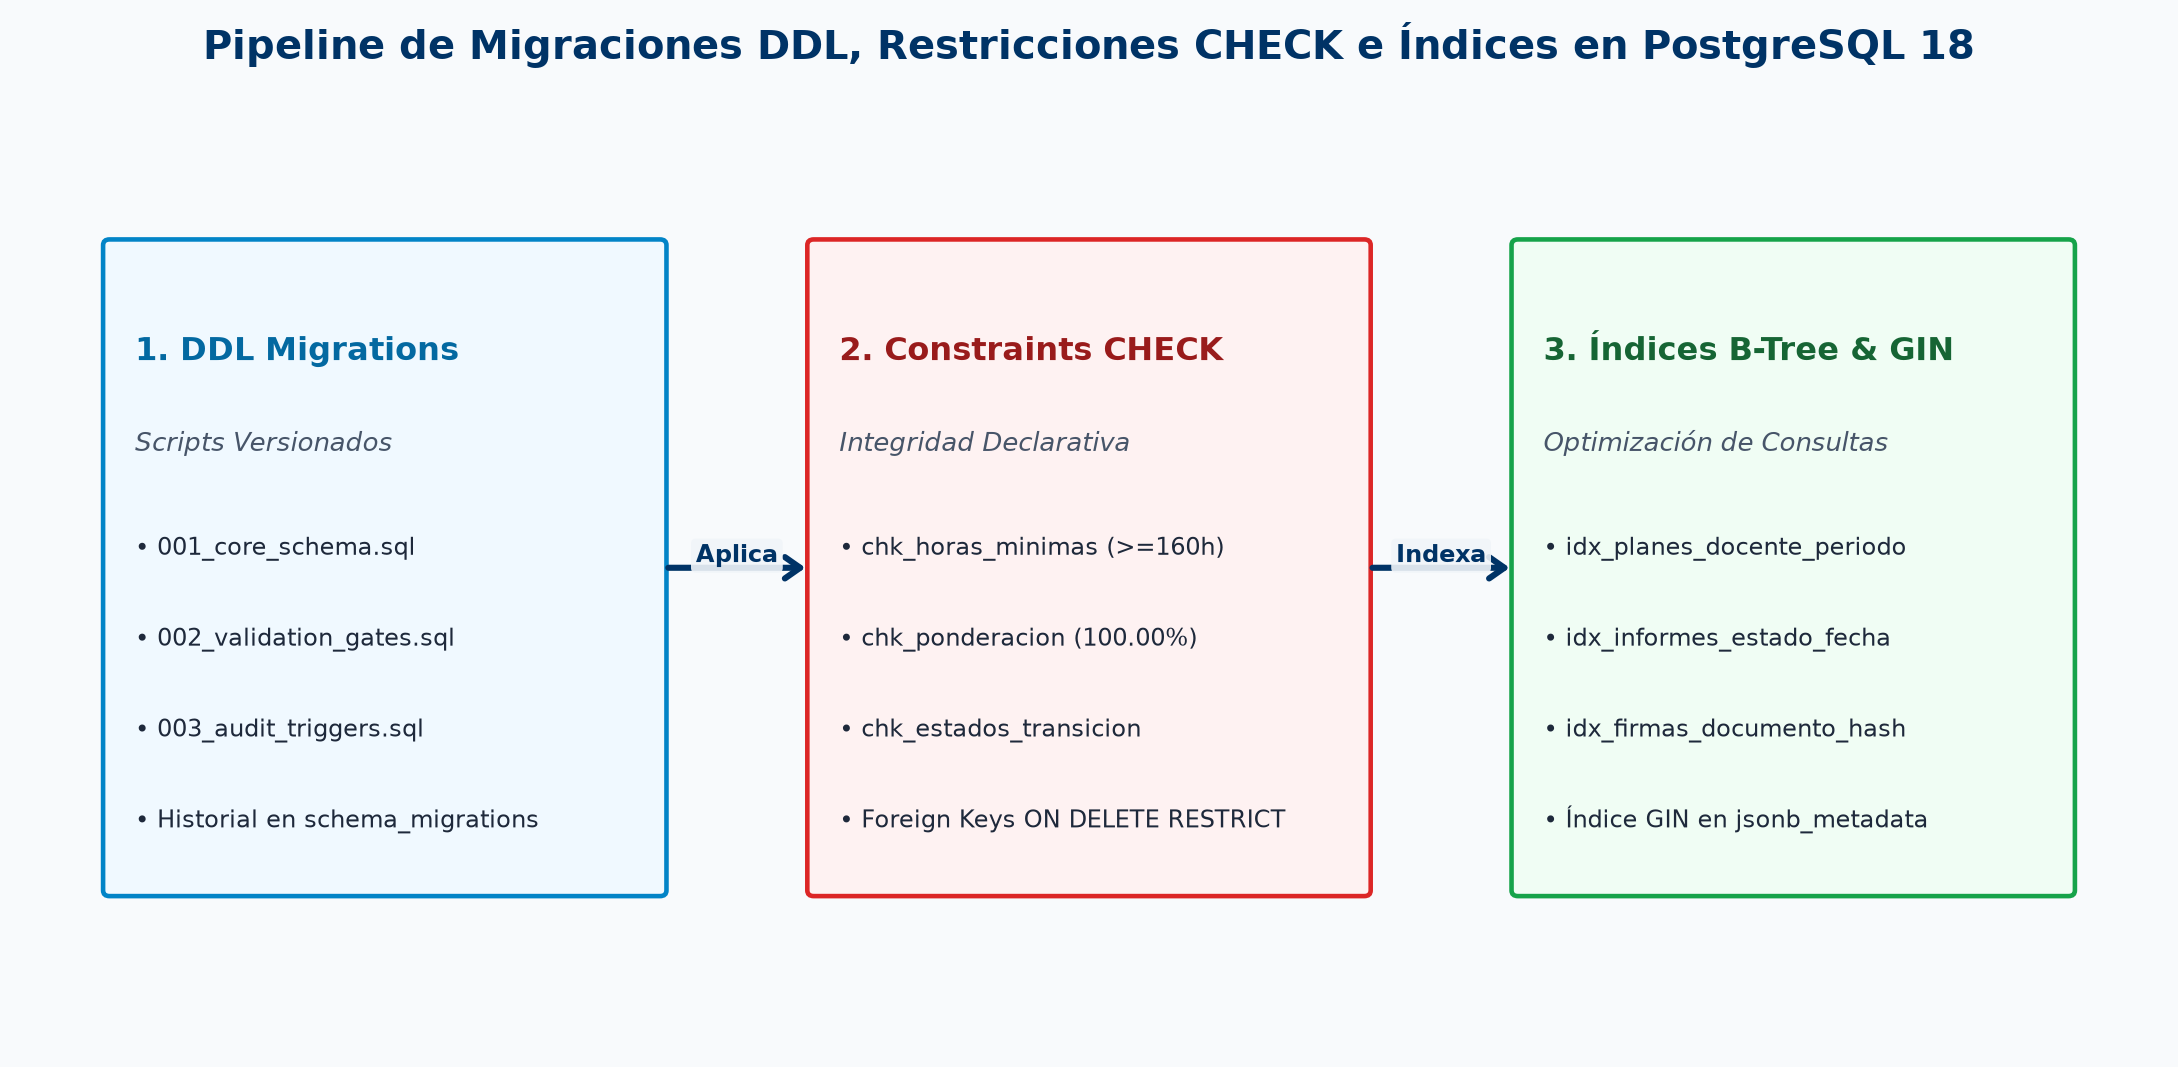
\includegraphics[width=0.88\textwidth,height=5.5cm,keepaspectratio]{images/f3_01_migraciones_indices_bd.png}
    \caption{Estructura Física de Tablas e Índices Relacionales en PostgreSQL 18.}
    \label{fig:f3_01_ddl}
\end{figure}

\section{Descripción de actividades}
\subsection{Catálogo Físico de Índices Implementados}
\begin{table}[htbp]
\centering
\small
\renewcommand{\arraystretch}{1.2}
\begin{tabularx}{\textwidth}{|>{\bfseries}m{3.5cm}|m{2.5cm}|m{3.5cm}|X|}
\hline
\rowcolor{tableheader}
\textbf{Nombre del Índice} & \textbf{Tabla Destino} & \textbf{Columnas Indexadas} & \textbf{Propósito y Tipo de Índice} \\
\hline
\texttt{idx\_doc\_usuario\_per} & \texttt{documentos} & \texttt{(usuario\_id, periodo\_id)} & B-Tree compuesto para acelerar la bandeja docente. \\
\hline
\texttt{idx\_doc\_estado} & \texttt{documentos} & \texttt{estado} & B-Tree para filtrar revisiones pendientes de coordinadores. \\
\hline
\texttt{idx\_act\_documento} & \texttt{actividades} & \texttt{documento\_id} & B-Tree para carga ágil de la Matriz Dinámica completa. \\
\hline
\texttt{idx\_evi\_actividad} & \texttt{evidencias} & \texttt{actividad\_id} & B-Tree para verificación rápida de anexos de actividad. \\
\hline
\texttt{idx\_sec\_doc\_orden} & \texttt{secciones} & \texttt{(documento\_id, orden)} & B-Tree para renderizado ordenado del Wizard. \\
\hline
\texttt{idx\_audit\_doc\_fecha} & \texttt{auditoria\_logs} & \texttt{(documento\_id, fecha)} & B-Tree compuesto para consultas de trazabilidad forense. \\
\hline
\end{tabularx}
\caption{Matriz de Índices Físicos y Optimización en PostgreSQL 18.}
\label{tab:indices_ddl}
\end{table}

\subsection{Verificación de Restricciones \texttt{CHECK}}
Se verificó el rechazo exitoso a nivel de motor ante intentos de inserción con ponderaciones menores a 0 o mayores a 100, y ante estados no catalogados, garantizando integridad física previa a la capa de aplicación.

\section{Firmas de Responsabilidad}

\noindent
\renewcommand{\arraystretch}{1.2}
\begin{tabularx}{\textwidth}{|>{\raggedright\arraybackslash}m{2.9cm}|>{\raggedright\arraybackslash}X|>{\centering\arraybackslash}m{4.6cm}|>{\centering\arraybackslash}m{2.3cm}|}
    \hline
    \rowcolor{tableheader}
    \textbf{ACCIÓN} & \textbf{NOMBRE Y CARGO} & \textbf{FIRMA} & \textbf{FECHA} \\
    \hline
    \textbf{Elaborado por:} & Heidi Villavicencio\newline Analista de Calidad / UI-UX & \parbox[c]{4.4cm}{\centering\vspace{4pt}
\includegraphics[height=1.5cm,width=4.0cm,keepaspectratio]{images/firma_heidi.png}\vspace{4pt}} & 10/09/2026 \\
    \hline
    \textbf{Revisado por:} & Steeven Toala\newline Líder de Proyecto / Arquitecto & \parbox[c]{4.4cm}{\centering\vspace{4pt}
\includegraphics[height=1.5cm,width=4.0cm,keepaspectratio]{images/firma_steveen.png}\vspace{4pt}} & 10/09/2026 \\
    \hline
    \textbf{Aprobado por:} & Ing. Paulo Torres, Mg.\newline Docente Evaluador -- Gestión Proyectos & \parbox[c]{4.4cm}{\centering\vspace{8pt}\textbf{\textcolor{gray!80}{\scriptsize [ PENDIENTE DE APROBACIÓN ]}}\vspace{8pt}} & \textbf{\textcolor{gray!90}{Pendiente}} \\
    \hline
\end{tabularx}

\vspace{0.4cm}

\section{Control de Cambios}

\noindent
\renewcommand{\arraystretch}{1.2}
\begin{tabularx}{\textwidth}{|>{\hsize=0.45\hsize\centering\arraybackslash}X|>{\hsize=1.55\hsize\raggedright\arraybackslash}X|>{\hsize=1.2\hsize\raggedright\arraybackslash}X|>{\hsize=0.8\hsize\centering\arraybackslash}X|}
    \hline
    \rowcolor{tableheader}
    \textbf{Versión} & \textbf{Descripción del cambio} & \textbf{Responsable del cambio} & \textbf{Fecha de aprobación} \\
    \hline
    1.0 & Emisión inicial del entregable según EDT del Tablero Trello & Equipo de Proyecto SIGE & 10/09/2026 \\
    \hline
\end{tabularx}

\vspace{0.4cm}

\section{Anexos}
\begin{itemize}[leftmargin=1.5em]
\item \textbf{Anexo 1:} Log de Ejecución de Scripts DDL en Contenedor PostgreSQL 18.
\end{itemize}

\end{document}
